\documentclass[11pt,a4paper]{article}
\usepackage[utf8]{inputenc}
\usepackage[T1]{fontenc}
\usepackage{amsfonts}
\usepackage[french]{babel}
\frenchbsetup{StandardLists=true} % à inclure si on utilise \usepackage[francais]{babel}
\usepackage{enumitem}
\usepackage{amssymb}
\usepackage{amsmath}
\usepackage[left=2cm,right=2cm,top=2cm,bottom=2cm]{geometry}
\usepackage[dvipsnames]{xcolor}

\usepackage[T1]{fontenc}
\usepackage{fouriernc}
\usepackage{graphicx}

\usepackage{setspace}
\singlespacing

\usepackage{pstricks}
\usepackage{xkeyval}
\usepackage{pst-labo}
\usepackage{colortbl}
\usepackage{tikz}
\usepackage{tikz-osci}

\usepackage{amssymb}
\usepackage{multicol}
\usepackage{caption}
\usepackage{fancyhdr}
\pagestyle{fancy}
\renewcommand\headrulewidth{1pt}
\fancyhead[L]{Lycée Denis Diderot }
\fancyhead[L]{Lycée Denis Diderot }
\fancyhead[R]{Classe de 1 Bac Pro }
\setcounter{page}{6}\fancyfoot[C]{page \thepage}
\fancyfoot[R]{Année 2024-2025}
\fancyfoot[L]{Alexis RUIZ}
\usepackage{multirow,tabularx,booktabs}
\newcommand{\cadreblanc}[1]{%
\medskip\framebox[\linewidth][c]{%
\rule{0mm}{#1mm}}\par
\medskip}

\usepackage{awesomebox}
\setlength{\aweboxvskip}{0mm}
\usepackage{pifont}
\usepackage{chemmacros}
\chemsetup{modules=all}
%\setlength{\columnseprule}{.25mm}

\renewcommand{\arraystretch}{3.5}
\newcolumntype{C}[1]{>{\centering\arraybackslash }b{#1}}

\newcommand*\acocher{\quitvmode{\fboxsep0pt \fboxrule0.8pt \fbox{\vrule height1.8ex depth.1ex width0pt \vrule height0pt depth0pt width1.9ex }}}

\newcommand{\code}{\awesomebox[black]{2pt}{

\includegraphics[scale=0.15]{../Chapitre 1 - Energie et puissance électrique/images/frame.png}
}{black}}

\newcommand{\moteur}{\awesomebox[black]{2pt}{

\includegraphics[scale=1]{images/moteur.jpg} 
}{black}}

\newcommand{\defconclusion}{\awesomebox[black]{2pt}{\rotatebox{90}{\Large{\textbf{Conclusion}}}}{black}}


  \newenvironment{itemize*}%  % listes compactes
    {\begin{itemize}%
      \setlength{\itemsep}{0pt}%
      \setlength{\parskip}{0pt}}%
    {\end{itemize}}


\frenchbsetup{StandardLists=true}


\frenchbsetup{StandardLists=true}
\newlist{fleche}{itemize}{1}
\setlist[fleche]{label=\ding{220},font=\color{orange}}

\AtBeginDocument{\shorthandoff{;}}

\begin{document}


\begin{center}
 \LARGE{Exercices } \\[3mm]
\end{center}



\normalsize

\hrule\
\\[0,5cm]


\fbox{\textbf{Exercice 1 }} QCM : Parmi les trois propositions, choisissez la bonne réponse. 

\begin{center}



    \begin{tabular}{|p{6cm}|C{3cm}|C{3cm}|C{3cm}|}
         \hline
       \ding{202} La puissance électrique $P_j$ s'exprime en ...& $\Box $ ~~watt& $\Box $ ~~kilowatt    & $\Box $ ~~Joule \\
         \hline
      \ding{203}La puissance électrique $P_j$ dissipée par effet Joule se calcule avec ...  & $\Box $ ~~$P_j=R \times I$ & $\Box $ ~~$P_j=R \times I^2$  & $\Box $ ~~ $P_j=R^2 \times I$ \\
         \hline
         \ding{204} Elle se calcule aussi avec ...  &$\Box $ ~~ $P_j=\dfrac{U}{R^2}$ & $\Box $ ~~ $P_j=\dfrac{U}{R}$  & $\Box $ ~~$P_j=\dfrac{U^2}{R}$  \\
         \hline
         \ding{205} Le rapport de transformation $m$ est donné par & $\Box $ ~~ $m=\dfrac{N_2}{N_1} $ & $\Box $ ~~ $m=\dfrac{N_1}{N_2} $ & $\Box $ ~~ $m=N_1 \times N_2 $ \\
         \hline
         \ding{206} Le rapport de transformation $m$ s'exprime ... &$\Box $ ~~ en Volt & $\Box $ ~~ sans unité & $\Box $ ~~ en Joule \\
         \hline
         \ding{207} Si~~$m=1$ alors ... & $\Box $ ~~ $U_2>U_1$ & $\Box $ ~~  $U_1>U_2$ & $\Box $ ~~  $U_1=U_2$ \\
         \hline
         %\ding{208} Un mouvement rectiligne uniformément ralenti peut être représenté par ...  & $\Box $ ~~  & $\Box $ ~~  &  $\Box $\\
         %\hline
         \ding{208} Si $m<1$ alors le transformateur est ... &$\Box$ ~~ abaisseur de tension & $\Box$ ~~ élévateur de tension &$\Box$ ~~ égaliseur de tension\\
         \hline
         \ding{209} Dans un transformateur parfait, on a ...  &$\Box ~~ \dfrac{U_1}{U_2}=\dfrac{I_2}{I_1}$ &$\Box ~~ \dfrac{U_2}{U_1}=\dfrac{I_2}{I_1}$  & $\Box ~~ \dfrac{U_2}{I_1}=\dfrac{I_2}{U_1}$ \\ 
         \hline 
         \ding{210} Le symbole électrique du transformateur est   &$\Box ~~ $ 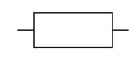
\includegraphics[scale=0.55]{images/QCM1.png}   &$\Box ~~ $ 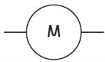
\includegraphics[scale=0.75]{images/QCM2.png}     &$\Box ~~ $ 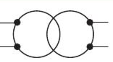
\includegraphics[scale=0.65]{images/QCM3.png}   \\
         \hline

         
        
    \end{tabular}
\end{center}
\vfill
\newpage

\fbox{\textbf{Exercice 2 }} Un transformateur considéré comme parfait a les caractéristiques suivantes : \\\begin{center}
220 V / 24 V - 50 Hz $\mathrm{N_1=700~spires}$.
\end{center}

\vfill 

\ding{202} Calculer le rapport de transformation $m$ 

\cadreblanc{20}

\vfill 

\ding{203} Combien y a-t-il de spires $\mathrm{N_2}$ au secondaire ? 

\cadreblanc{20}

\vfill 

\fbox{\textbf{Exercice 3 }} 
\begin{center}
Pour chaque situation, indiquez si le transformateur est élévateur ou abaisseur de tension, et calculer son rapport de transformation. 
\end{center}

\vfill 

\ding{202} Un poste de transformation électrique 20 kV/400 V placé à l'entrée d'un lotissement. 

\cadreblanc{20}

\vfill 

\ding{203} Un transformateur  reçoit une tension de 23 V et la transforme en tension de 15 kV. 

\cadreblanc{20}

\vfill 

\ding{204} Un transformateur d'isolement 230 V / 230 V sécurise un local de travail 

\cadreblanc{15}

\vfill 


\newpage 

\fbox{\textbf{Exercice 4 }} \\[8mm]

Un transformateur supposé parfait est utilisé pour l'alimentation des lampes d'un garage.  La tension efficace au primaire est de 220 V. 

\begin{enumerate}


\item Afin de déterminer la nature du transformateur , on visualise à l'aide de l'oscilloscope, la tension aux bornes du circuit secondaire. 

\begin{center}
    
\osci[%
scale=1,
second channel=0, %1 pour activer la deuxième voie, 0 sinon.
screen offset one=0, %Décalage vertical de la voie 1 sur l’écran
screen offset two=0, %Décalage vertical de la voie 2 sur l’écran
time div=10, %Durée par division (en ms)
voltage div one=2, %Tension par division (en V) pour la voie 1
voltage div two=2, %Tension par division (en V) pour la voie 2
sample rate=200, %Taux d’échantillonnage
xy mode=0, %1 pour l’activer, 0 sinon 
func one=6.8*sin(2*180/0.050*x),
func two=3*sin(2*180/0.020*x+180), %+ 0.2*sin(2*180/0.040*x),
color one=D62626, %Couleur de la voie 1 (en hexadecimal)
color two=1053AF, %Couleur de la voie 2 (en hexadecimal)
graph back color=FFFFFF,
info back color=D6D6D6,
info text color=000000,
main axis color=000000,
grid color=CCCCCC
]

\end{center}


    1.1. Déterminer, en volt, la valeur maximale $U_{max}$ de la tension au secondaire. 

    \cadreblanc{10}

    1.2. En déduire, en volt, la valeur efficace $U_{eff}$ de cette tension (arrondir le résultat à l'unité). 

    \cadreblanc{15}

    \item Calculer $m$ , le rapport de transformation 

    \cadreblanc{15}

    \item Le transformateur est-il élévateur ou abaisseur de tension :

    \vspace{8mm}

    \dotfill 
    


\end{enumerate}

\newpage 




\end{document}